\hypertarget{native_2lwip_2src_2core_2ipv4_2etharp_8c}{}\section{/home/ayush/\+R\+I\+O\+T/tests/lwip/bin/pkg/native/lwip/src/core/ipv4/etharp.c File Reference}
\label{native_2lwip_2src_2core_2ipv4_2etharp_8c}\index{/home/ayush/\+R\+I\+O\+T/tests/lwip/bin/pkg/native/lwip/src/core/ipv4/etharp.\+c@{/home/ayush/\+R\+I\+O\+T/tests/lwip/bin/pkg/native/lwip/src/core/ipv4/etharp.\+c}}
{\ttfamily \#include \char`\"{}lwip/opt.\+h\char`\"{}}\newline
Include dependency graph for etharp.\+c\+:
\nopagebreak
\begin{figure}[H]
\begin{center}
\leavevmode
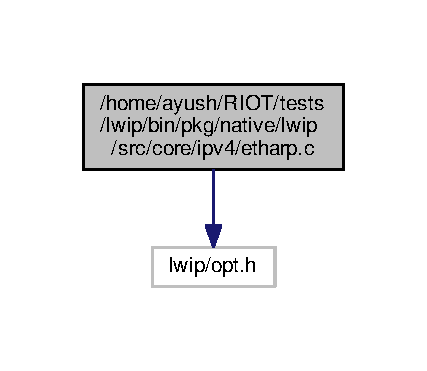
\includegraphics[width=205pt]{native_2lwip_2src_2core_2ipv4_2etharp_8c__incl}
\end{center}
\end{figure}


\subsection{Detailed Description}
Address Resolution Protocol module for IP over Ethernet

Functionally, A\+RP is divided into two parts. The first maps an IP address to a physical address when sending a packet, and the second part answers requests from other machines for our physical address.

This implementation complies with R\+FC 826 (Ethernet A\+RP). It supports Gratuitious A\+RP from R\+F\+C3220 (IP Mobility Support for I\+Pv4) section 4.\+6 if an interface calls etharp\+\_\+gratuitous(our\+\_\+netif) upon address change. 